%% AI Test Agent — Minor Project Report
%% Pandit Deendayal Energy University
%% Compile with: pdflatex -> biber -> pdflatex -> pdflatex
%%=============================================================================

\documentclass[12pt,a4paper,oneside]{report}

%%=============================================================================
%% PACKAGES
%%=============================================================================

% Page geometry
\usepackage[top=1in, bottom=1in, left=1.5in, right=1in]{geometry}

% Font — Times New Roman equivalent for pdfLaTeX
\usepackage[T1]{fontenc}
\usepackage{newtxtext}
\usepackage{newtxmath}

% Line spacing
\usepackage{setspace}
\onehalfspacing

% Graphics
\usepackage{graphicx}
\graphicspath{{images/}{diagrams/}}

% TikZ and diagrams
\usepackage{tikz}
\usetikzlibrary{
  positioning,
  arrows.meta,
  shapes.geometric,
  shapes.multipart,
  fit,
  calc,
  backgrounds,
  matrix,
  chains,
  decorations.pathreplacing,
  decorations.markings
}
\usepackage{pgfplots}
\pgfplotsset{compat=1.18}

% Tables
\usepackage{booktabs}
\usepackage{longtable}
\usepackage{array}
\usepackage{tabularx}
\usepackage{multirow}

% Floats
\usepackage{float}

% Captions
\usepackage{caption}
\usepackage{subcaption}
\captionsetup{font={small}, labelfont={bf}, skip=8pt}

% Lists
\usepackage{enumitem}

% Colors
\usepackage[dvipsnames,table]{xcolor}

% Headers and footers
\usepackage{fancyhdr}

% Chapter and section title formatting
\usepackage{titlesec}

% Hyperlinks
\usepackage[
  colorlinks=true,
  linkcolor=black,
  citecolor=black,
  urlcolor=blue,
  bookmarks=true,
  bookmarksnumbered=true
]{hyperref}

% Bibliography
\usepackage[
  backend=biber,
  style=numeric,
  sorting=nyt,
  maxbibnames=99
]{biblatex}
\addbibresource{references.bib}

% Code listings
\usepackage{listings}
\lstset{
  basicstyle=\ttfamily\small,
  breaklines=true,
  frame=single,
  numbers=left,
  numberstyle=\tiny\color{gray},
  keywordstyle=\color{blue},
  commentstyle=\color{green!50!black},
  stringstyle=\color{red!70!black},
  showstringspaces=false,
  tabsize=2,
  captionpos=b
}

% PDF metadata
\usepackage{pdfpages}

% Misc
\usepackage{url}
\usepackage{csquotes}
\usepackage{pdflscape}

%%=============================================================================
%% CUSTOM COMMANDS AND STYLES
%%=============================================================================

% Project details
\newcommand{\projecttitle}{AI Test Agent: Autonomous AI-Based Web Application Testing and Intelligent Bug Reporting}
\newcommand{\studentname}{Meet Prajapati}
\newcommand{\rollnumber}{23BCP265}
\newcommand{\department}{Computer Engineering}
\newcommand{\guidename}{[Name of Guide]}
\newcommand{\guidedesignation}{[Designation]}
\newcommand{\academicyear}{2025}
\newcommand{\examinername}{[Name of Examiner]}
\newcommand{\examinerdesignation}{[Designation]}

% TikZ common styles used across diagrams
\tikzset{
  service/.style={
    rectangle,
    rounded corners=4pt,
    draw=MidnightBlue,
    fill=MidnightBlue!10,
    text=black,
    minimum width=3cm,
    minimum height=1cm,
    align=center,
    font=\small\bfseries
  },
  database/.style={
    cylinder,
    cylinder uses custom fill,
    cylinder body fill=Cerulean!15,
    cylinder end fill=Cerulean!25,
    draw=Cerulean!70!black,
    shape border rotate=90,
    minimum width=2cm,
    minimum height=1cm,
    align=center,
    font=\small
  },
  process/.style={
    rectangle,
    rounded corners=3pt,
    draw=RoyalBlue!80!black,
    fill=RoyalBlue!8,
    text=black,
    minimum width=3.5cm,
    minimum height=0.9cm,
    align=center,
    font=\small
  },
  decision/.style={
    diamond,
    draw=Orange!80!black,
    fill=Orange!10,
    text=black,
    minimum width=2cm,
    minimum height=1.5cm,
    align=center,
    font=\small,
    aspect=2
  },
  external/.style={
    rectangle,
    draw=ForestGreen!80!black,
    fill=ForestGreen!8,
    text=black,
    minimum width=2.8cm,
    minimum height=0.9cm,
    align=center,
    font=\small
  },
  user/.style={
    rectangle,
    rounded corners=6pt,
    draw=Maroon!80!black,
    fill=Maroon!8,
    text=black,
    minimum width=2.5cm,
    minimum height=0.9cm,
    align=center,
    font=\small\bfseries
  },
  arrow/.style={
    -Stealth[length=3mm],
    thick,
    color=MidnightBlue!70!black
  },
  dashedarrow/.style={
    -Stealth[length=3mm],
    thick,
    dashed,
    color=gray!70
  },
  label/.style={
    font=\scriptsize,
    text=MidnightBlue!80!black
  }
}

%%=============================================================================
%% HEADER / FOOTER
%%=============================================================================

\pagestyle{fancy}
\fancyhf{}
\fancyhead[L]{\small\leftmark}
\fancyhead[R]{\small\thepage}
\fancyfoot[C]{\small Department of \department, PDEU}
\renewcommand{\headrulewidth}{0.4pt}
\renewcommand{\footrulewidth}{0.4pt}

% Plain style for chapter opening pages
\fancypagestyle{plain}{
  \fancyhf{}
  \fancyfoot[C]{\small\thepage}
  \renewcommand{\headrulewidth}{0pt}
  \renewcommand{\footrulewidth}{0.4pt}
}

%%=============================================================================
%% TITLE FORMATTING
%%=============================================================================

\titleformat{\chapter}[display]
  {\normalfont\Large\bfseries\centering}
  {\chaptertitlename\ \thechapter}{14pt}{\LARGE}
\titlespacing*{\chapter}{0pt}{-20pt}{30pt}

\titleformat{\section}
  {\normalfont\large\bfseries}{\thesection}{1em}{}
\titleformat{\subsection}
  {\normalfont\normalsize\bfseries}{\thesubsection}{1em}{}
\titleformat{\subsubsection}
  {\normalfont\normalsize\itshape}{\thesubsubsection}{1em}{}

%%=============================================================================
%% DOCUMENT BEGIN
%%=============================================================================
\begin{document}

%%-----------------------------------------------------------------------------
%% PRELIMINARY PAGES (Roman numerals, no headers on cover/title/cert)
%%-----------------------------------------------------------------------------
\pagenumbering{gobble}

% Cover Page (Color)
%%=============================================================================
%% COVER PAGE (Color version — printed on card stock)
%%=============================================================================
\thispagestyle{empty}

\begin{center}

\vspace*{0.5cm}

{\Large \textbf{A Seminar Report}}

\vspace{0.3cm}

{\large on}

\vspace{0.5cm}

{\LARGE \textbf{\projecttitle}}

\vspace{1.2cm}

{\large by}

\vspace{0.5cm}

{\Large \textbf{\studentname}}

\vspace{0.2cm}

{\large \rollnumber}

\vspace{1.0cm}

{\large Under the Guidance of}

\vspace{0.3cm}

{\large \textbf{\guidename}}

\vspace{0.1cm}

{\large \guidedesignation}

\vspace{1.2cm}

% University Logo
\IfFileExists{images/pdeu_logo.png}{%
  \includegraphics[width=3cm]{images/pdeu_logo.png}%
}{%
  % Placeholder if logo is not available
  
\begin{tikzpicture}
    \draw[thick, MidnightBlue] (0,0) circle (1.3cm);
    \node[align=center, font=\small\bfseries, text=MidnightBlue] at (0,0) {PDEU\\Logo};
  \end{tikzpicture}%
}

\vspace{1.0cm}

{\large Submitted to}

\vspace{0.3cm}

{\large \textbf{Department of \department}}

\vspace{0.2cm}

{\large School of Technology}

\vspace{0.2cm}

{\large \textbf{Pandit Deendayal Energy University}}

\vspace{0.2cm}

{\large Gandhinagar}

\vspace{0.8cm}

{\large \academicyear}

\end{center}

\newpage

% Title Page (Black and White)
%%=============================================================================
%% TITLE PAGE (Black and White version)
%%=============================================================================
\thispagestyle{empty}

\begin{center}

\vspace*{0.5cm}

{\Large \textbf{A Seminar Report}}

\vspace{0.3cm}

{\large on}

\vspace{0.5cm}

{\LARGE \textbf{\projecttitle}}

\vspace{1.2cm}

{\large by}

\vspace{0.5cm}

{\Large \textbf{\studentname}}

\vspace{0.2cm}

{\large \rollnumber}

\vspace{1.0cm}

{\large Under the Guidance of}

\vspace{0.3cm}

{\large \textbf{\guidename}}

\vspace{0.1cm}

{\large \guidedesignation}

\vspace{1.2cm}

% University Logo (B&W)
\IfFileExists{images/pdeu_logo.png}{%
  \includegraphics[width=3cm]{images/pdeu_logo.png}%
}{%
  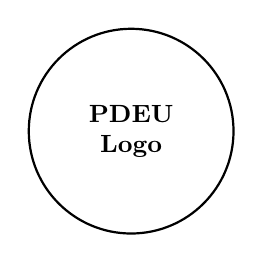
\begin{tikzpicture}
    \draw[thick, black] (0,0) circle (1.3cm);
    \node[align=center, font=\small\bfseries] at (0,0) {PDEU\\Logo};
  \end{tikzpicture}%
}

\vspace{1.0cm}

{\large Submitted to}

\vspace{0.3cm}

{\large \textbf{Department of \department}}

\vspace{0.2cm}

{\large School of Technology}

\vspace{0.2cm}

{\large \textbf{Pandit Deendayal Energy University}}

\vspace{0.2cm}

{\large Gandhinagar}

\vspace{0.8cm}

{\large \academicyear}

\end{center}

\newpage

% Certificate
%%=============================================================================
%% CERTIFICATE (Appendix 2 format)
%%=============================================================================
\thispagestyle{empty}

\begin{center}
{\Large \textbf{CERTIFICATE}}
\end{center}

\vspace{1.5cm}

\begin{spacing}{1.8}
\noindent
This is to certify that the seminar report entitled ``\projecttitle,'' submitted by \textbf{\studentname{} (\rollnumber)}, has been conducted under the supervision of \textbf{\guidename}, \textbf{\guidedesignation}, and is hereby approved for the partial fulfillment of the requirements for the award of the degree of Bachelor of Engineering in the Department of \department{} at Pandit Deendayal Energy University, Gandhinagar. This work is original and has not been submitted to any other institution for the award of any degree.
\end{spacing}

\vspace{3cm}

\noindent
\begin{minipage}[t]{0.45\textwidth}
\textbf{Sign:} \hrulefill \\[0.5cm]
\textbf{\guidename} \\
\guidedesignation \\
Department of \department \\
School of Technology \\
Pandit Deendayal Energy University
\end{minipage}
\hfill
\begin{minipage}[t]{0.45\textwidth}
\textbf{Sign:} \hrulefill \\[0.5cm]
\textbf{\examinername} \\
\examinerdesignation \\
Department of \department \\
School of Technology \\
Pandit Deendayal Energy University
\end{minipage}

\newpage

% AI Declaration
%%=============================================================================
%% DECLARATION FOR USING AI TOOLS (Appendix 3 — Truthful version)
%%=============================================================================
\thispagestyle{empty}

\begin{center}
{\Large \textbf{DECLARATION}}
\end{center}

\vspace{1.0cm}

\begin{spacing}{1.8}
\noindent
I hereby declare that the seminar report entitled ``\projecttitle'' is the result of my own work and effort. The project described in this report, including the system design, architecture, and implementation, was independently developed by me.

\vspace{0.5cm}

\noindent
In preparing this report document, AI-based language model tools were used to assist with structuring the report content, refining technical descriptions, generating \LaTeX{} formatting and diagrams, and improving the overall presentation quality. The underlying project work, including the system architecture design, microservices implementation, database design, AI integration logic, and Playwright-based browser automation, was carried out independently.

\vspace{0.5cm}

\noindent
This declaration is to transparently affirm the nature and extent of AI assistance used in the preparation of this report, subject to university guidelines and approval.
\end{spacing}

\vspace{1.5cm}

\noindent
\textbf{\studentname} \\
\rollnumber \\
Department of \department \\
School of Technology \\
Pandit Deendayal Energy University \\
Gandhinagar

\vspace{1.0cm}

\noindent
\textbf{Date:} \hrulefill \\[0.4cm]
\textbf{Place:} Gandhinagar

\vspace{1.0cm}

\noindent
\textbf{List of AI Tools Used for the Report with Purpose:}

\begin{enumerate}[leftmargin=2cm]
  \item \textbf{Claude (Anthropic):} Assistance with report structuring, technical writing, \LaTeX{} formatting, and TikZ diagram generation.
  \item \textbf{Antigravity (Google):} Agentic coding assistant used for \LaTeX{} project compilation and automation.
\end{enumerate}

\newpage

%%-----------------------------------------------------------------------------
%% Switch to Roman numbering for remaining preliminaries
%%-----------------------------------------------------------------------------
\pagenumbering{roman}
\setcounter{page}{1}

% Acknowledgement
%%=============================================================================
%% ACKNOWLEDGEMENT
%%=============================================================================
\chapter*{Acknowledgement}
\addcontentsline{toc}{chapter}{Acknowledgement}

\begin{spacing}{1.8}
I would like to express my sincere gratitude to all those who contributed to the successful completion of this minor project.

First and foremost, I extend my heartfelt thanks to my project guide, \textbf{\guidename}, \guidedesignation, Department of \department, School of Technology, Pandit Deendayal Energy University, for providing valuable guidance, encouragement, and constructive feedback throughout the course of this project. Their mentorship was instrumental in shaping the direction and quality of this work.

I am grateful to the \textbf{Department of \department}, School of Technology, Pandit Deendayal Energy University, Gandhinagar, for providing the academic environment and resources necessary for undertaking this project.

I would also like to thank the faculty members of the department for their insightful suggestions during project reviews, which helped refine the system design and implementation approach.

Finally, I express my appreciation to my peers and family for their continuous support and encouragement during the development of this project.

\vspace{1.5cm}

\noindent
\textbf{\studentname} \\
\rollnumber \\
Department of \department \\
School of Technology \\
Pandit Deendayal Energy University
\end{spacing}

\newpage

% Abstract
%%=============================================================================
%% ABSTRACT
%%=============================================================================
\chapter*{Abstract}
\addcontentsline{toc}{chapter}{Abstract}

\begin{spacing}{1.8}
Software testing is a critical phase in the software development lifecycle, responsible for ensuring the quality, reliability, and correctness of web applications. Traditional manual testing approaches require significant human effort to understand application workflows, design test cases, execute them against the application, identify failures, and produce detailed bug reports. These processes are time-consuming, error-prone, and difficult to scale as application complexity increases.

Existing automated testing tools, while effective for executing predefined scripts, still depend on human testers to analyze the application, identify meaningful workflows, and author test cases. Recent advances in artificial intelligence, particularly large language models (LLMs) and agentic AI systems, present an opportunity to bridge this gap by introducing intelligent reasoning capabilities into the testing pipeline.

This project presents \textbf{AI Test Agent}, an autonomous AI-based web application testing and intelligent bug reporting platform developed using a microservices architecture. The system accepts a target web application URL and autonomously performs the complete testing workflow: exploration, test generation, execution, failure detection, and bug reporting.

The platform consists of seven logically independent microservices: an \textbf{Authentication Service} for secure user management with JWT-based authentication, an \textbf{API Gateway} built with Spring Cloud Gateway for centralized request routing, a \textbf{Service Registry} using Eureka for dynamic service discovery, an \textbf{Exploration Service} that uses Playwright to inspect the target application and discover pages, links, buttons, forms, and input fields, a \textbf{Test/AI Service} that communicates with an LLM to understand discovered workflows and generate structured functional test cases, an \textbf{Execution Service} that uses Playwright to perform browser-based test execution with assertion validation and evidence capture, and a \textbf{Bug Analysis Service} that employs an LLM to analyze failed executions and generate structured, developer-friendly bug reports.

A key architectural principle of this system is the clear separation of AI reasoning and deterministic browser automation. The LLM performs cognitive tasks such as workflow understanding, test scenario generation, and failure analysis, while Playwright handles all actual browser interactions including navigation, form filling, clicking, assertion verification, and screenshot capture. This combination of AI reasoning with deterministic execution produces reliable and interpretable testing outcomes.

The system was implemented using React.js for the frontend dashboard, Java with Spring Boot for the backend microservices, PostgreSQL with a database-per-service pattern, and Git for version control. The implemented platform demonstrates the feasibility of autonomous, AI-driven web application testing as an integrated end-to-end solution.
\end{spacing}

\newpage

% Table of Contents
\tableofcontents
\newpage

% List of Tables
\listoftables
\newpage

% List of Figures
\listoffigures
\newpage

% Abbreviations
%%=============================================================================
%% LIST OF ABBREVIATIONS
%%=============================================================================
\chapter*{List of Symbols, Abbreviations, and Nomenclature}
\addcontentsline{toc}{chapter}{List of Abbreviations}

\begin{longtable}{@{}p{3.5cm} p{10cm}@{}}
\toprule
\textbf{Abbreviation} & \textbf{Full Form} \\
\midrule
\endhead

AI      & Artificial Intelligence \\
API     & Application Programming Interface \\
BCrypt  & Blowfish Crypt (Password Hashing Algorithm) \\
CI/CD   & Continuous Integration / Continuous Deployment \\
CORS    & Cross-Origin Resource Sharing \\
CSS     & Cascading Style Sheets \\
DB      & Database \\
DOM     & Document Object Model \\
GUI     & Graphical User Interface \\
HTML    & HyperText Markup Language \\
HTTP    & HyperText Transfer Protocol \\
IDE     & Integrated Development Environment \\
JSON    & JavaScript Object Notation \\
JWT     & JSON Web Token \\
LLM     & Large Language Model \\
MVP     & Minimum Viable Product \\
NLP     & Natural Language Processing \\
PDEU    & Pandit Deendayal Energy University \\
REST    & Representational State Transfer \\
SDLC    & Software Development Life Cycle \\
SQL     & Structured Query Language \\
SUT     & System Under Test \\
TDD     & Test-Driven Development \\
UI      & User Interface \\
UML     & Unified Modeling Language \\
URL     & Uniform Resource Locator \\
UX      & User Experience \\
XSS     & Cross-Site Scripting \\

\bottomrule
\end{longtable}

\newpage

%%-----------------------------------------------------------------------------
%% MAIN CHAPTERS (Arabic numerals)
%%-----------------------------------------------------------------------------
\pagenumbering{arabic}
\setcounter{page}{1}

% ============================================================
% Chapter 1: Introduction
% AI Test Agent — Minor Project Report, PDEU
% Author: Meet Prajapati (23BCP265)
% ============================================================

\chapter{Introduction}
\label{chap:intro}

The rapid proliferation of web-based applications across virtually every sector of industry and governance has fundamentally altered the landscape of software engineering. As organizations increasingly rely on complex, feature-rich web platforms to deliver services, process transactions, and engage with users, the imperative to ensure the correctness, reliability, and security of these systems has never been more critical. Software testing, long regarded as an indispensable phase of the Software Development Life Cycle (SDLC), has struggled to keep pace with the velocity of modern agile and DevOps-driven development workflows. Traditional manual testing methodologies, while thorough in their intent, suffer from inherent limitations in speed, scalability, and consistency that render them inadequate for the demands of contemporary software delivery pipelines.

This chapter introduces the \textbf{AI Test Agent}, an autonomous, artificial-intelligence-driven web application testing and intelligent bug reporting platform built upon a microservices architecture. The system leverages Large Language Models (LLMs) for cognitive reasoning about application behaviour, the Playwright browser automation framework for reliable cross-browser interaction, and a distributed service-oriented backend to deliver end-to-end automated testing without the need for manually authored test scripts. The following sections establish the background, motivation, problem statement, objectives, and scope of this project, and conclude with an overview of the system architecture and the organization of the remainder of this report.


% ============================================================
\section{Background}
\label{sec:background}

The World Wide Web has evolved from a medium for static document retrieval into a sophisticated application delivery platform. Modern web applications---ranging from enterprise resource planning systems and e-commerce marketplaces to healthcare portals and financial trading dashboards---are characterised by dynamic content rendering, complex client-side logic executed within JavaScript frameworks, asynchronous server communication via RESTful and GraphQL APIs, and rich user interface (UI) components such as modals, drag-and-drop interfaces, infinite scroll regions, and single-page application (SPA) navigation patterns.

According to industry estimates, the global count of active websites exceeded 1.1 billion by 2024, with web application complexity growing at an exponential rate driven by the adoption of frameworks such as React, Angular, and Vue.js on the frontend and microservices-based backends powered by Spring Boot, Node.js, and Django~\cite{playwright2024}. This complexity has profound implications for quality assurance (QA). A single modern web application may expose hundreds of distinct user-facing routes, each containing dozens of interactive elements whose behaviour depends on application state, user roles, network conditions, and browser-specific rendering engines.

The traditional approach to ensuring quality---wherein human testers manually navigate through the application, verify expected behaviours, and document defects---is increasingly untenable. The gap between the rate at which new features are developed and deployed (often multiple times per day in continuous deployment pipelines) and the rate at which those features can be manually verified has widened to a critical degree. Automated testing frameworks such as Selenium~\cite{selenium2004} and, more recently, Playwright~\cite{playwright2024} have partially bridged this gap by enabling programmatic browser control. However, these tools require significant human effort to author, maintain, and update test scripts---effort that scales linearly with application complexity.

The advent of powerful Large Language Models (LLMs) such as GPT-4~\cite{openai2023gpt4}, built upon the Transformer architecture~\cite{vaswani2017attention}, has opened an entirely new frontier. These models demonstrate remarkable capabilities in understanding natural language descriptions of software behaviour, reasoning about UI semantics from structural representations such as the Document Object Model (DOM), and generating syntactically and semantically correct test code. The AI Test Agent project was conceived at the intersection of these technological currents: leveraging LLM-based reasoning to autonomously understand web application workflows and generate executable test cases, while utilising Playwright for deterministic, real-browser test execution.


% ============================================================
\section{Software Testing Overview}
\label{sec:testing_overview}

Software testing is a systematic process of evaluating a software system or its components to verify that it satisfies specified requirements and to identify defects~\cite{istqb2023}. It is an integral part of the SDLC and serves as the primary mechanism for quality assurance. The IEEE Standard 829~\cite{ieee829} defines software testing documentation standards that govern how test plans, test cases, and test reports are structured in professional practice.

Software testing can be classified along several dimensions. The most fundamental classification is based on the \emph{level} of testing, which corresponds to the granularity of the system component under test:

\begin{enumerate}
    \item \textbf{Unit Testing:} Unit testing focuses on verifying the correctness of individual units of source code---typically functions, methods, or classes---in isolation from the rest of the system. Unit tests are authored by developers and are executed frequently during development, often as part of continuous integration pipelines. Frameworks such as JUnit (Java), pytest (Python), and Jest (JavaScript) are widely used for unit testing. The primary advantage of unit testing lies in its ability to localise defects to specific code units, enabling rapid diagnosis and correction.

    \item \textbf{Integration Testing:} Integration testing examines the interactions between integrated units or modules to detect interface defects. After individual units have been verified, integration testing ensures that they function correctly when combined. This level of testing is particularly important in microservices architectures, where services communicate via network protocols (HTTP, gRPC, message queues), and subtle issues such as data format mismatches, authentication failures, or timeout behaviours may emerge only when services interact.

    \item \textbf{System Testing:} System testing evaluates the complete, integrated system against its specified requirements. It is conducted in an environment that closely mirrors the production deployment and covers both functional requirements (e.g., ``the user can successfully submit a registration form'') and non-functional requirements (e.g., performance under load, security against common vulnerabilities). System testing treats the application as a black box, exercising it through its external interfaces---primarily the user interface for web applications.

    \item \textbf{Acceptance Testing:} Acceptance testing determines whether the system meets the acceptance criteria defined by stakeholders and is ready for deployment. User Acceptance Testing (UAT) involves end users or their representatives exercising the system in realistic scenarios. In agile methodologies, acceptance criteria are often expressed as user stories with associated acceptance tests that must pass before a feature is considered complete.
\end{enumerate}

Beyond the level-based classification, testing is also categorised by \emph{approach}:

\begin{itemize}
    \item \textbf{Black-Box Testing:} Tests are designed based on the external specification of the system without knowledge of its internal implementation. Techniques include equivalence partitioning, boundary value analysis, and state transition testing.
    \item \textbf{White-Box Testing:} Tests are designed with knowledge of the internal code structure. Techniques include statement coverage, branch coverage, and path coverage analysis.
    \item \textbf{Grey-Box Testing:} A hybrid approach that combines elements of both black-box and white-box testing, often used in integration and security testing.
\end{itemize}

Furthermore, testing encompasses specialised types such as \textbf{regression testing} (re-executing tests after code changes to ensure no existing functionality is broken), \textbf{smoke testing} (a preliminary test to verify that the most critical functions work), \textbf{performance testing} (evaluating system responsiveness and stability under load), and \textbf{security testing} (identifying vulnerabilities such as SQL injection, cross-site scripting, and authentication bypasses).

The AI Test Agent project operates primarily at the \textbf{system testing} level, treating the web application under test as a black box and interacting with it through its browser-rendered user interface. The system autonomously generates and executes functional test cases that verify user-facing workflows, thereby addressing the most labour-intensive and time-consuming tier of the testing pyramid.


% ============================================================
\section{Traditional Manual Testing}
\label{sec:manual_testing}

Traditional manual testing involves human testers directly interacting with the software application to identify defects, verify functionality, and validate that the system meets its requirements. Despite the growing adoption of automation, manual testing remains prevalent across the industry, particularly for exploratory testing, usability evaluation, and testing of novel features where automated scripts do not yet exist.

The manual testing process typically follows a structured workflow:

\begin{enumerate}
    \item \textbf{Test Planning:} A test manager or lead creates a test plan that defines the scope, approach, resources, schedule, and deliverables of the testing effort. The test plan identifies the features to be tested, the testing techniques to be employed, and the entry and exit criteria for each testing phase, in accordance with standards such as IEEE 829~\cite{ieee829}.

    \item \textbf{Test Case Design:} QA engineers analyse requirements documents, user stories, and design specifications to derive test cases. Each test case specifies a unique identifier, preconditions, input data, a sequence of test steps, expected results, and postconditions. For a web application, a typical test case might specify: ``Navigate to the login page, enter valid credentials, click the Submit button, and verify that the user is redirected to the dashboard.''

    \item \textbf{Test Environment Setup:} The test environment---including the application server, database, network configuration, and browser versions---is configured to replicate the production environment as closely as possible. Environment discrepancies are a common source of false positives and false negatives in testing.

    \item \textbf{Test Execution:} Testers manually execute each test case by following the prescribed steps, interacting with the application through its user interface, and observing the actual outcomes. The tester compares the actual result with the expected result and records the outcome as Pass or Fail.

    \item \textbf{Defect Reporting:} When a test case fails, the tester creates a defect report (bug report) that includes the defect summary, severity, priority, steps to reproduce, expected versus actual behaviour, screenshots or screen recordings, and environment details. Bug reports are submitted to a defect tracking system such as Jira, Bugzilla, or Azure DevOps.

    \item \textbf{Regression Testing:} After developers fix reported defects, testers re-execute the failed test cases to verify the fix and also re-execute a broader set of test cases to ensure that the fix has not introduced new defects (regression). This cycle of fix--verify--regress is repeated until the exit criteria are met.
\end{enumerate}

The human roles involved in manual testing include \textbf{QA Analysts} (who design test cases), \textbf{QA Engineers/Testers} (who execute tests), \textbf{Test Leads/Managers} (who plan and coordinate testing activities), and \textbf{Business Analysts/Product Owners} (who define acceptance criteria). In many organisations, a single individual may fulfil multiple roles.

Manual testing offers certain undeniable advantages: human testers possess intuition, domain knowledge, and the ability to detect subtle usability and aesthetic issues that automated tools cannot easily identify. Exploratory testing---an approach wherein the tester simultaneously learns about the application, designs tests, and executes them---relies heavily on human judgement and creativity.

However, as discussed in the following section, the limitations of manual testing become severe as application complexity and release frequency increase.


% ============================================================
\section{Challenges in Existing Testing Approaches}
\label{sec:challenges}

Both manual testing and traditional script-based automated testing face significant challenges that impede the efficiency and effectiveness of quality assurance in modern web development:

\subsection{Time-Intensive Nature of Manual Testing}
\label{subsec:time_intensive}

Manual test execution is inherently slow. A human tester can execute at most a few dozen test cases per day for a complex web application, whereas a modern continuous integration pipeline may produce multiple new builds daily. The time required to manually regress an entire application after each build is prohibitive, leading to either delayed releases or insufficient test coverage. Studies in the testing literature indicate that manual regression testing can consume up to 60--80\% of the total testing effort in large projects~\cite{istqb2023}.

\subsection{Human Error and Inconsistency}
\label{subsec:human_error}

Manual testing is susceptible to human error. Testers may inadvertently skip test steps, misinterpret expected results, or fail to notice subtle UI anomalies due to fatigue or cognitive overload. Furthermore, different testers may execute the same test case in slightly different ways, leading to inconsistent results. This variability undermines the repeatability and reliability of the testing process.

\subsection{Scalability Limitations}
\label{subsec:scalability}

As the application under test grows in size and complexity, the number of test cases required to achieve adequate coverage grows combinatorially. Manual testing does not scale: doubling the number of features approximately doubles (or more) the number of test cases and the time required to execute them. Cross-browser testing (verifying behaviour across Chrome, Firefox, Safari, and Edge) and cross-device testing (desktop, tablet, mobile) further multiply the testing matrix.

\subsection{Test Script Maintenance Burden}
\label{subsec:maintenance}

Traditional automated testing tools such as Selenium~\cite{selenium2004} address the speed and consistency limitations of manual testing by enabling programmatic browser control. However, they introduce a new challenge: \textbf{test script maintenance}. Automated test scripts are tightly coupled to the application's UI structure---element locators (CSS selectors, XPaths, IDs) become invalid whenever the UI is refactored, causing tests to fail even when the underlying functionality is correct. Studies report that test maintenance can consume 40--60\% of the total automation effort, often negating the productivity gains of automation.

\subsection{Repetitive and Monotonous Nature}
\label{subsec:repetitive}

Regression testing, by its very definition, involves the repeated execution of the same test cases across successive builds. This repetitive work is demotivating for skilled QA professionals and represents an inefficient utilisation of human cognitive resources. The monotony contributes to decreased attention and increased error rates over time.

\subsection{Limited Adaptability to UI Changes}
\label{subsec:adaptability}

Traditional automated tests are brittle in the face of UI changes. A simple refactoring of the HTML structure---such as changing a \texttt{<div>} to a \texttt{<section>} or renaming a CSS class---can break dozens of automated test scripts simultaneously. The effort required to update these scripts after each UI change discourages teams from maintaining comprehensive automated test suites, leading to a gradual erosion of automated test coverage.

\subsection{Lack of Intelligent Failure Analysis}
\label{subsec:failure_analysis}

When a traditional automated test fails, it typically produces a generic error message (e.g., ``Element not found'' or ``Assertion failed''). Diagnosing the root cause requires manual investigation by a developer or QA engineer, who must examine screenshots, log files, and application state to understand why the failure occurred. This diagnostic process is time-consuming and requires significant domain expertise.

The AI Test Agent addresses each of these challenges through its autonomous, AI-driven approach: LLM-based reasoning enables adaptive understanding of UI structure without brittle selectors; autonomous exploration eliminates the need for manually authored test scripts; real-browser execution via Playwright ensures consistent, repeatable test runs; and AI-powered failure analysis produces intelligent, context-rich bug reports that accelerate defect resolution.


% ============================================================
\section{Motivation}
\label{sec:motivation}

The motivation for the AI Test Agent project arises from a fundamental asymmetry in the current state of AI-assisted software engineering. Over the past several years, AI-powered code generation tools---such as GitHub Copilot, Amazon CodeWhisperer, and ChatGPT---have dramatically accelerated the speed at which software is written. Developers routinely use LLMs to generate boilerplate code, implement algorithms, and even scaffold entire application modules. This acceleration in code production has further compressed release cycles and intensified the pressure on QA teams.

However, a conspicuous gap exists on the \emph{testing} side of the development workflow. While AI has been extensively applied to code generation, its application to \emph{autonomous testing}---the ability to independently explore a web application, understand its workflows, generate test cases, execute them, and report failures---remains nascent. Most existing AI-assisted testing tools focus on narrow tasks such as generating unit tests for individual functions or predicting which tests are likely to fail. Few, if any, provide end-to-end autonomous testing of web applications at the system level.

This gap creates a dangerous imbalance: code is produced faster than it can be tested, leading to increased defect escape rates, degraded software quality, and elevated technical debt. The AI Test Agent was developed to close this gap by bringing the same level of AI-powered autonomy to testing that already exists for code generation.

Several converging technological enablers made this project feasible:

\begin{itemize}
    \item \textbf{Advances in Large Language Models:} The release of GPT-4~\cite{openai2023gpt4} and similar models demonstrated that LLMs can reason about complex, structured inputs such as HTML DOM trees, understand the semantic purpose of UI elements (e.g., distinguishing a login form from a registration form), and generate syntactically correct Playwright test scripts from natural-language descriptions of expected behaviour.

    \item \textbf{Mature Browser Automation Frameworks:} Playwright~\cite{playwright2024} provides a modern, reliable API for controlling Chromium, Firefox, and WebKit browsers. Unlike earlier tools such as Selenium~\cite{selenium2004}, Playwright offers auto-waiting for elements, network interception, and native support for modern web features such as Shadow DOM, iframes, and single-page application routing.

    \item \textbf{Microservices Architecture Patterns:} The widespread adoption of microservices architecture patterns, service discovery (Eureka), API gateways, and containerised deployments enables the construction of distributed systems with clear separation of concerns, independent scalability, and fault isolation---all of which are essential for a production-grade testing platform.

    \item \textbf{The Transformer Architecture:} The Transformer architecture~\cite{vaswani2017attention}, which underpins modern LLMs, provides the attention mechanism necessary for processing long-context inputs such as full-page DOM snapshots and generating coherent, contextually appropriate test code.
\end{itemize}

The AI Test Agent was therefore motivated by the need to create an \emph{intelligent, autonomous testing platform} that eliminates the manual effort of test case authoring, adapts to UI changes without script maintenance, and provides AI-powered defect analysis---thereby restoring the balance between the velocity of modern software development and the rigour of quality assurance.


% ============================================================
\section{Problem Statement}
\label{sec:problem_statement}

The increasing complexity of modern web applications, coupled with the accelerating pace of software releases driven by agile and DevOps methodologies, has rendered traditional manual and script-based automated testing approaches inadequate. Manual testing is too slow, error-prone, and labour-intensive to keep pace with continuous delivery pipelines. Script-based automated testing, while faster, imposes a significant maintenance burden due to the tight coupling between test scripts and the application's UI structure, leading to brittle test suites that break with every UI change.

Formally, the problem addressed by this project is stated as follows:

\begin{quote}
\emph{Design and develop an autonomous, AI-driven web application testing platform that can independently explore a target web application, understand its user-facing workflows through intelligent analysis of UI structure, automatically generate functional test cases, execute them in real browser environments, classify test outcomes, and produce detailed, AI-analysed bug reports---without requiring manually authored test scripts or human intervention during the testing process.}
\end{quote}

The system must satisfy the following constraints:
\begin{itemize}
    \item The platform must operate on any publicly accessible web application, without requiring access to the application's source code or internal APIs.
    \item Test generation and failure analysis must be performed by AI (LLM-based reasoning), not by rule-based heuristics alone.
    \item Browser interaction must be performed through a real browser automation framework (Playwright), not through simulated HTTP requests, ensuring that client-side rendering, JavaScript execution, and dynamic content loading are accurately represented.
    \item The system must be architected as a set of independently deployable microservices to ensure scalability, maintainability, and fault isolation.
\end{itemize}


% ============================================================
\section{Objectives}
\label{sec:objectives}

The AI Test Agent project was developed with the following six primary objectives:

\begin{enumerate}
    \item \textbf{Automated Web Application Exploration:} Develop an exploration engine capable of autonomously crawling a target web application, discovering its pages, routes, and interactive elements (links, buttons, forms, navigation menus), and constructing a structured representation of the application's UI topology. The exploration engine uses real-browser navigation via Playwright to handle dynamic content, JavaScript-rendered pages, and single-page application routing.

    \item \textbf{AI-Driven Workflow Understanding:} Leverage Large Language Models to analyse the explored UI structure and infer meaningful user workflows. Given the DOM structure, element attributes, labels, and page context, the LLM identifies logical user journeys---such as login flows, registration processes, search operations, and form submissions---and determines the sequence of interactions required to complete each workflow.

    \item \textbf{AI-Powered Test Case Generation:} Utilise LLM-based reasoning to automatically generate executable test cases for the identified workflows. Each generated test case includes a descriptive title, a sequence of browser interaction steps (navigation, clicking, typing, selecting, asserting), expected outcomes, and appropriate assertions. The generated tests are expressed as Playwright-compatible code that can be directly executed without manual modification.

    \item \textbf{Real Browser Test Execution via Playwright:} Execute the generated test cases in real browser environments using the Playwright framework~\cite{playwright2024}. The execution engine launches browser instances, runs each test case by performing the specified interactions, captures screenshots at key steps, records console logs and network requests, and collects execution metadata including timing information and browser version.

    \item \textbf{Intelligent Failure Detection and Classification:} Implement a robust test outcome classification system that categorises each test execution into one of four states: \textbf{PASS} (all assertions succeeded), \textbf{FAIL} (one or more assertions did not hold), \textbf{TIMEOUT} (the test exceeded its maximum allowed execution time), or \textbf{ERROR} (an unexpected exception occurred during execution, such as a browser crash or network failure). This classification provides immediate, actionable feedback on the health of the application.

    \item \textbf{Automated Intelligent Bug Reporting:} For test cases that result in FAIL, TIMEOUT, or ERROR outcomes, automatically generate comprehensive bug reports using AI-powered analysis. The bug reports include a summary of the failure, the specific step at which the failure occurred, the expected versus actual behaviour, severity assessment, potential root cause analysis, and remediation suggestions---all produced by LLM reasoning over the test execution context, screenshots, and error logs.
\end{enumerate}


% ============================================================
\section{Scope of the Project}
\label{sec:scope}

The scope of the AI Test Agent project is defined by the following inclusions and exclusions:

\subsection{In Scope}
\label{subsec:in_scope}

\begin{itemize}
    \item \textbf{Functional UI Testing:} The system performs functional testing of web application user interfaces, verifying that user-facing workflows behave as expected. This includes testing form submissions, navigation flows, authentication processes, search functionality, and CRUD (Create, Read, Update, Delete) operations.

    \item \textbf{Cross-Browser Support:} Test execution supports Chromium-based browsers through Playwright, with the architecture designed to extend to Firefox and WebKit.

    \item \textbf{Autonomous Operation:} The system operates autonomously from exploration through test execution and bug reporting, without requiring manually authored test scripts or real-time human supervision.

    \item \textbf{AI-Powered Analysis:} LLMs are used for workflow understanding, test case generation, and failure analysis. The system supports integration with OpenAI-compatible LLM APIs.

    \item \textbf{Microservices Architecture:} The backend is architected as a set of seven microservices with clear separation of concerns, service discovery via Eureka, and API gateway routing.

    \item \textbf{Web-Based Dashboard:} A React-based frontend provides users with the ability to initiate testing sessions, monitor progress, view test results, and review generated bug reports.

    \item \textbf{Persistent Data Storage:} Test configurations, exploration results, generated test cases, execution outcomes, and bug reports are persisted in PostgreSQL databases.
\end{itemize}

\subsection{Out of Scope}
\label{subsec:out_of_scope}

\begin{itemize}
    \item \textbf{Performance and Load Testing:} The system does not perform performance benchmarking, stress testing, or load testing of the target application.

    \item \textbf{Security Testing:} Specialised security testing activities such as penetration testing, vulnerability scanning, and fuzzing are not included, although the system may incidentally detect certain security-related UI behaviours.

    \item \textbf{Mobile Application Testing:} The system is designed for web applications rendered in desktop and responsive web browsers; native mobile application testing (iOS/Android) is not supported.

    \item \textbf{API-Level Testing:} The system tests applications through their browser-rendered user interfaces, not through direct API invocation. API contract testing and integration testing at the API level are outside the scope.

    \item \textbf{Source Code Analysis:} The system operates as a black-box testing tool and does not analyse or require access to the target application's source code.

    \item \textbf{Test Data Generation for Domain-Specific Applications:} While the system generates generic test inputs (e.g., email addresses, passwords, names), it does not generate domain-specific test data (e.g., valid insurance policy numbers or medical record identifiers).
\end{itemize}


% ============================================================
\section{Overview of AI Test Agent}
\label{sec:system_overview}

The AI Test Agent is a full-stack, microservices-based platform that automates the entire web application testing lifecycle---from exploration and understanding through test generation, execution, and intelligent bug reporting. The system architecture, as shown in Figure~\ref{fig:system_architecture}, comprises seven backend microservices, a React-based frontend application, PostgreSQL databases for persistent storage, the Playwright browser automation framework for real-browser interaction, and integration with LLM APIs for AI-powered reasoning.

A central architectural principle of the AI Test Agent is the \textbf{separation of reasoning from interaction}: the AI (LLM) performs all cognitive tasks---understanding application structure, inferring workflows, generating test logic, and analysing failures---while Playwright handles all browser-level interactions---navigating to URLs, clicking elements, filling forms, capturing screenshots, and observing page state. This separation ensures that the AI's reasoning capabilities are leveraged where they provide the greatest value, while browser interaction remains deterministic and reliable.

The seven backend microservices are:

\begin{enumerate}
    \item \textbf{Authentication Service (Auth Service):} Manages user registration, authentication, and JWT-based authorisation. All API requests are authenticated through this service, ensuring secure access to the platform's functionality.

    \item \textbf{API Gateway:} Serves as the single entry point for all client requests. The gateway performs request routing, load balancing, and cross-cutting concerns such as rate limiting and CORS handling. It routes requests to the appropriate downstream microservice based on the URL path and HTTP method.

    \item \textbf{Service Discovery (Eureka Server):} Implements the service registry pattern using Netflix Eureka. Each microservice registers itself with the Eureka server upon startup and discovers other services dynamically, enabling location-transparent inter-service communication without hard-coded hostnames or ports.

    \item \textbf{Exploration Service:} Responsible for autonomously crawling and exploring the target web application. The service launches a Playwright browser instance, navigates through the application's pages, extracts DOM structure, identifies interactive elements (links, buttons, forms, input fields), and records the application's page topology. The exploration results are persisted and provided as input to the test generation phase.

    \item \textbf{Test Generation and AI Service (Test/AI Service):} Receives the exploration results and uses LLM-based reasoning to understand the application's workflows and generate executable test cases. The service constructs carefully engineered prompts that include the DOM structure, element attributes, page context, and workflow descriptions, and sends these prompts to an LLM API (e.g., GPT-4~\cite{openai2023gpt4}). The LLM's response---a set of test cases with step-by-step browser interactions and assertions---is parsed, validated, and stored.

    \item \textbf{Execution Service:} Executes the generated test cases in real Playwright browser instances. For each test case, the service launches a browser, performs the specified sequence of interactions (navigate, click, type, select, assert), captures screenshots at critical steps, records console output and network activity, measures execution time, and classifies the outcome as PASS, FAIL, TIMEOUT, or ERROR. Execution results, including all captured artefacts, are persisted for review and analysis.

    \item \textbf{Bug Analysis Service:} Processes test executions that resulted in non-PASS outcomes. The service collects the test case definition, execution logs, error messages, screenshots, and page state at the point of failure, and submits this context to an LLM for intelligent failure analysis. The LLM generates a structured bug report that includes a failure summary, root cause hypothesis, severity assessment, affected workflow, and suggested remediation steps. These reports are stored and presented to the user through the frontend dashboard.
\end{enumerate}

The \textbf{React frontend} provides a modern, responsive single-page application through which users interact with the platform. Key frontend features include project configuration (specifying the target URL and authentication credentials), real-time exploration progress monitoring, test case review and editing, test execution dashboards with pass/fail statistics, and detailed bug report viewing with associated screenshots and logs.

\textbf{PostgreSQL} serves as the primary relational database management system, with each microservice maintaining its own database schema in accordance with the database-per-service pattern recommended for microservices architectures. This isolation ensures that schema changes in one service do not affect others and enables independent data management.

The overall testing workflow proceeds as follows: the user specifies a target web application URL through the React frontend; the Exploration Service autonomously crawls the application and builds a structural map; the Test/AI Service analyses the exploration data using an LLM and generates test cases; the Execution Service runs the test cases in Playwright browsers and records results; and the Bug Analysis Service generates intelligent bug reports for any failures. The entire pipeline operates autonomously once initiated, with results presented to the user upon completion.


% ============================================================
\section{Organization of the Report}
\label{sec:report_organization}

The remainder of this report is organised as follows:

\begin{itemize}
    \item \textbf{Chapter~\ref{chap:litsurvey}: Literature Survey} reviews the existing body of work in automated software testing, AI-assisted testing, browser automation frameworks, and LLM-based code generation. The chapter analyses the strengths and limitations of prior approaches and identifies the research gaps that the AI Test Agent addresses.

    \item \textbf{Chapter~\ref{chap:methodology}: Methodology} describes the software development methodology adopted for the project, including the agile development process, microservices design principles, and the AI pipeline architecture. The chapter also details the system requirements---both functional and non-functional---and the technology stack selection rationale.

    \item \textbf{Chapter~\ref{chap:design}: System Design} presents the detailed architectural design of the AI Test Agent, including the high-level system architecture, individual microservice designs, database schema designs, API specifications, and the interaction patterns between services. UML diagrams including use case diagrams, sequence diagrams, and component diagrams are provided.

    \item \textbf{Chapter~\ref{chap:implementation}: Implementation} documents the implementation details of each microservice and the frontend application, including key code structures, algorithm descriptions, LLM prompt engineering strategies, Playwright integration patterns, and inter-service communication mechanisms.

    \item \textbf{Chapter~\ref{chap:results}: Results and Discussion} presents the outcomes of testing the AI Test Agent on sample web applications, including exploration coverage metrics, test generation quality analysis, execution pass/fail distributions, and bug report accuracy assessments. The chapter discusses the system's strengths, limitations, and observations.

    \item \textbf{Chapter~\ref{chap:conclusion}: Conclusion and Future Work} summarises the contributions of the project, reflects on the objectives achieved, discusses the limitations encountered, and outlines directions for future enhancement---including support for additional LLM providers, visual regression testing, and CI/CD pipeline integration.
\end{itemize}


%% ============================================================================
%% Chapter 2 — Literature Survey
%% AI Test Agent: Autonomous AI-Based Web Application Testing
%%                and Intelligent Bug Reporting
%% ============================================================================

\chapter{Literature Survey}
\label{chap:litsurvey}

This chapter presents a comprehensive review of the literature that underpins the
design and development of the AI Test Agent platform. The survey spans classical
software testing theory, modern automated testing frameworks, the emergence of
artificial intelligence and large language models (LLMs) in software engineering,
agentic AI paradigms, browser automation technologies, intelligent bug detection
research, and microservices-based software architecture. A comparative analysis
of existing tools and approaches is provided, culminating in an identification of
the research gap that the AI Test Agent addresses.

%%=============================================================================
\section{Introduction to Software Testing Research}
\label{sec:testing_research_intro}
%%=============================================================================

Software testing is a systematic process of evaluating a software system to
detect differences between existing and required conditions and to assess the
features of the software~\cite{myers2011art}. It is universally acknowledged as
one of the most critical activities in the software development life cycle
(SDLC), consuming an estimated 30--50\% of total project effort in
industrial practice~\cite{aniche2022testing}. The International Software
Testing Qualifications Board (ISTQB) defines testing as the process consisting
of all life cycle activities, both static and dynamic, concerned with planning,
preparation, and evaluation of a component or system and related work products
to determine that they satisfy specified requirements~\cite{istqb2023}.

Historically, software testing research has evolved through several distinct
phases. Early work in the 1970s and 1980s established the theoretical
foundations of test adequacy criteria, including statement coverage, branch
coverage, and path coverage~\cite{myers2011art}. The 1990s and 2000s saw the
maturation of automated test execution frameworks and the formalization of
model-based testing. The 2010s brought data-driven approaches, with machine
learning being applied to test case prioritization, fault prediction, and
automated test generation. Most recently, the 2020s have witnessed a
paradigm shift with the introduction of large language models capable of
understanding and generating both natural language and source
code~\cite{openai2023gpt4, chen2021codex}.

The AI Test Agent project is situated at this modern intersection of software
testing, agentic AI systems, and LLM-driven reasoning. It draws upon decades
of testing theory while leveraging the latest advances in AI to create an
autonomous testing platform that observes, reasons about, plans, and executes
functional tests on web applications without manual test script authoring.

%%=============================================================================
\section{Traditional Software Testing Techniques}
\label{sec:traditional_testing}
%%=============================================================================

Traditional software testing techniques form the bedrock upon which all
subsequent automation and AI-driven approaches are built. These techniques
are broadly categorized by the degree of internal knowledge available to
the tester.

\subsection{Black-Box Testing}
\label{subsec:black_box}

Black-box testing, also called specification-based testing, treats the system
under test as an opaque entity and derives test cases entirely from the
external specification~\cite{myers2011art}. The tester has no knowledge of or
access to the internal code structure. Key black-box techniques include:

\begin{itemize}[nosep]
  \item \textbf{Equivalence Partitioning:} The input domain is divided into
        classes of data from which test cases are derived, under the
        assumption that all members of a partition are processed equivalently.
  \item \textbf{Boundary Value Analysis:} Test cases are designed at the
        edges of equivalence partitions, as experience shows that errors
        tend to cluster at boundaries.
  \item \textbf{Decision Table Testing:} Combinatorial logic involving
        multiple conditions and their corresponding actions is captured
        in a decision table, from which test cases are systematically derived.
  \item \textbf{State Transition Testing:} The system is modeled as a finite
        state machine, and tests exercise transitions between states triggered
        by events and guarded by conditions.
\end{itemize}

The AI Test Agent employs a form of black-box testing in its core workflow:
the exploration service crawls the target application's user interface to
discover navigable elements, forms, buttons, and links. The LLM-based test
planner then generates functional test cases based solely on the observed
UI structure and inferred application semantics, without access to the
target application's source code.

\subsection{White-Box Testing}
\label{subsec:white_box}

White-box testing, or structural testing, leverages full knowledge of the
internal implementation to design test cases that exercise specific code
paths~\cite{myers2011art}. Techniques include statement coverage, branch
coverage, condition coverage, and path coverage. While white-box testing
achieves thorough code-level verification, it requires access to source
code and deep understanding of the implementation, making it impractical
for external or third-party application testing scenarios.

\subsection{Gray-Box Testing}
\label{subsec:gray_box}

Gray-box testing combines elements of both black-box and white-box
approaches. The tester possesses partial knowledge of the internal
structure---such as data flow, architectural patterns, or API
contracts---while designing tests that are executed from the external
interface. The AI Test Agent can be considered a gray-box approach in
the sense that the exploration service extracts structural information
(DOM elements, form structures, navigation patterns) from the
target application, providing the AI planner with partial internal
knowledge beyond what a pure black-box tester would possess.

\subsection{Regression Testing}
\label{subsec:regression}

Regression testing ensures that previously working functionality continues
to operate correctly after code changes, bug fixes, or feature
additions~\cite{istqb2023}. It is one of the most resource-intensive
testing activities, as the regression suite tends to grow monotonically
over the life of a project. Test case prioritization and selection
techniques have been extensively studied to manage regression testing
costs~\cite{aniche2022testing}. The AI Test Agent contributes to this
domain by enabling rapid regeneration of test suites for target
applications---since tests are generated autonomously from the current
UI state, the system naturally adapts to interface changes without
manual test maintenance.

%%=============================================================================
\section{Automated Functional Testing}
\label{sec:automated_testing}
%%=============================================================================

Automated functional testing involves the use of specialized software
tools to control the execution of tests and the comparison of actual
outcomes with predicted outcomes. This section reviews the major
frameworks and paradigms in web application test automation.

\subsection{Selenium}
\label{subsec:selenium}

Selenium is the most widely adopted open-source web testing
framework~\cite{selenium2004}. It provides the WebDriver API, which
enables programmatic control of web browsers (Chrome, Firefox, Edge,
Safari) through language bindings in Java, Python, C\#, JavaScript,
and Ruby. Selenium's architecture is based on a client--server model
where the WebDriver client sends commands to a browser-specific driver
binary, which translates them into browser-native automation protocols.

While Selenium revolutionized web testing, it has well-documented
limitations: flaky tests due to implicit timing dependencies, lack of
built-in auto-waiting mechanisms, difficulty handling modern single-page
application (SPA) frameworks, limited support for intercepting network
requests, and the overhead of managing separate driver binaries for each
browser version.

\subsection{Cypress}
\label{subsec:cypress}

Cypress emerged as a developer-centric alternative to Selenium,
executing tests directly within the browser's JavaScript runtime rather
than over a remote protocol. This in-process architecture provides
deterministic execution, automatic waiting, time-travel debugging, and
real-time reloading. However, Cypress is limited to Chromium-based
browsers and Firefox, does not support multi-tab or multi-domain testing
in a single test, and is restricted to the JavaScript/TypeScript
ecosystem.

\subsection{Playwright}
\label{subsec:playwright_overview}

Microsoft Playwright represents the latest generation of browser
automation libraries~\cite{playwright2024}. It supports Chromium,
Firefox, and WebKit from a single API, provides built-in auto-waiting,
network interception, and multiple browser context isolation. Playwright
is available in JavaScript/TypeScript, Python, Java, and .NET. Its
architecture communicates with browsers over the Chrome DevTools Protocol
(CDP) and equivalent protocols for Firefox and WebKit, enabling
fine-grained control over browser behavior. The AI Test Agent uses
Playwright for Java as its deterministic browser actuator, as discussed
further in Section~\ref{sec:playwright_detail}.

\subsection{Record-and-Playback vs.\ Script-Based Approaches}
\label{subsec:record_playback}

Record-and-playback tools (e.g., Selenium IDE, Playwright Codegen)
capture user interactions and replay them as automated tests. While
accessible to non-programmers, these tools produce brittle, hard-to-maintain
scripts that break with minor UI changes. Script-based approaches, where
engineers manually author test code using framework APIs, offer greater
flexibility and maintainability but require significant programming
expertise and time investment. The AI Test Agent transcends both paradigms:
it autonomously generates test plans from observed UI structure using LLM
reasoning, then executes them through Playwright's programmatic API---combining
the accessibility of record-and-playback with the robustness of
script-based execution.

%%=============================================================================
\section{Artificial Intelligence in Software Testing}
\label{sec:ai_testing}
%%=============================================================================

The application of artificial intelligence techniques to software testing
has been an active research area for over two decades, with significant
acceleration in recent years.

\subsection{Machine Learning for Test Case Generation}
\label{subsec:ml_test_gen}

Machine learning (ML) models have been applied to generate test cases
from various software artifacts. Supervised learning approaches train
models on historical test data to predict effective test inputs.
Reinforcement learning agents have been used to explore application
state spaces, learning optimal sequences of UI interactions that
maximize code coverage or fault detection~\cite{aniche2022testing}.
Search-based software testing (SBST) employs evolutionary algorithms
(genetic algorithms, particle swarm optimization) to evolve test suites
that optimize coverage criteria. Tools such as EvoSuite for Java unit
testing exemplify this approach, generating JUnit test suites that
achieve high branch coverage through guided search.

\subsection{Test Case Prioritization}
\label{subsec:test_prioritization}

Test case prioritization reorders test suites to maximize the rate of
fault detection, enabling earlier discovery of defects in time-constrained
testing environments~\cite{istqb2023}. ML-based prioritization
techniques use features such as code change history, test execution
history, code complexity metrics, and requirement traceability to predict
which tests are most likely to reveal faults. Deep learning models,
including recurrent neural networks, have been applied to learn temporal
patterns in test failure histories for improved prioritization accuracy.

\subsection{Fault Localization}
\label{subsec:fault_localization}

Fault localization identifies the most probable locations of defects in
source code, given a set of failing and passing test cases.
Spectrum-based fault localization (SBFL) techniques, such as Tarantula,
Ochiai, and DStar, rank program statements by suspiciousness scores
computed from test execution spectra. ML-enhanced fault localization
models incorporate additional features---such as code complexity,
developer change patterns, and code churn---to improve localization
accuracy. The AI Test Agent's bug analysis service applies a
complementary approach: rather than analyzing source code spectra, it
uses LLM-based reasoning over execution traces, failure screenshots, and
assertion results to generate root-cause hypotheses in natural language.

\subsection{Mutation Testing}
\label{subsec:mutation_testing}

Mutation testing evaluates test suite quality by introducing small
syntactic changes (mutants) into the source code and measuring the
proportion of mutants detected (killed) by the test
suite~\cite{aniche2022testing}. While computationally expensive, mutation
testing provides a rigorous measure of test effectiveness. AI techniques
have been applied to reduce mutation testing costs through equivalent
mutant detection and selective mutation strategies.

%%=============================================================================
\section{Large Language Models in Software Engineering}
\label{sec:llm_se}
%%=============================================================================

The emergence of large language models (LLMs) has fundamentally
transformed multiple aspects of software engineering, from code
generation to testing to documentation.

\subsection{Transformer Architecture and the GPT Family}
\label{subsec:transformers}

The transformer architecture, introduced by Vaswani et
al.~\cite{vaswani2017attention}, replaced recurrent neural networks
with self-attention mechanisms that process input sequences in parallel.
This architecture enabled the training of models on vastly larger
datasets, leading to emergent capabilities in language understanding
and generation. The Generative Pre-trained Transformer (GPT) family
of models, culminating in GPT-4~\cite{openai2023gpt4}, demonstrated
state-of-the-art performance across a wide range of natural language
processing and code-related tasks. GPT-4 is a multimodal model capable
of accepting both text and image inputs, producing text outputs with
human-level performance on numerous professional and academic
benchmarks.

\subsection{Code Generation with LLMs}
\label{subsec:code_gen}

OpenAI Codex, a GPT model fine-tuned on publicly available code
repositories, demonstrated that LLMs can generate functionally correct
code from natural language descriptions~\cite{chen2021codex}. Chen et
al.\ evaluated Codex on the HumanEval benchmark, a set of 164 Python
programming problems, achieving 28.8\% pass@1 accuracy with the initial
model, rising to 72.3\% with 100 samples (pass@100). Subsequent models
(GPT-3.5-turbo, GPT-4) substantially improved these numbers. The
capability to generate code from natural language is foundational to
the AI Test Agent's approach: the LLM receives structured descriptions
of discovered web pages and generates executable test plans expressed
as sequences of browser actions.

\subsection{Test Generation with LLMs}
\label{subsec:llm_test_gen}

Recent research has explored the use of LLMs for automated test
generation~\cite{king2024llmtest}. Studies demonstrate that LLMs can
generate unit tests, integration tests, and end-to-end tests from
source code, documentation, or UI descriptions. Key findings include:

\begin{itemize}[nosep]
  \item LLMs generate tests with reasonable code coverage, though they
        may produce tests with incorrect assertions (hallucinated oracles).
  \item Prompt engineering---including few-shot examples, chain-of-thought
        reasoning, and structured output formatting---significantly
        improves test quality.
  \item LLM-generated tests are most effective when combined with
        deterministic execution and validation, as the AI Test Agent
        does by separating LLM-based planning from Playwright-based
        execution.
\end{itemize}

The AI Test Agent builds on this research direction by using LLMs not
merely to generate isolated test functions but to reason about
end-to-end user workflows across multiple pages, producing structured
JSON test plans that are validated and executed deterministically.

%%=============================================================================
\section{Agentic AI Systems}
\label{sec:agentic_ai}
%%=============================================================================

Agentic AI refers to systems where an AI model operates as an
autonomous agent that perceives its environment, reasons about
observations, plans actions, and executes those actions in a feedback
loop~\cite{yang2023agentic, wang2024survey}. This paradigm extends
beyond single-query LLM usage into multi-step, goal-directed behavior.

\subsection{Autonomous Agents and Cognitive Architectures}
\label{subsec:autonomous_agents}

Wang et al.~\cite{wang2024survey} present a comprehensive survey on
LLM-based autonomous agents, identifying four key modules: profiling,
memory, planning, and action. The profiling module defines the agent's
role and expertise. The memory module maintains short-term (context
window) and long-term (external storage) information. The planning
module decomposes complex tasks into sub-goals through strategies such
as chain-of-thought reasoning, task decomposition, and self-reflection.
The action module translates plans into concrete operations in the
external environment.

\subsection{Observe--Reason--Act Loops}
\label{subsec:ora_loop}

The observe--reason--act (ORA) loop is the fundamental execution cycle
of an agentic AI system. At each iteration, the agent:

\begin{enumerate}[nosep]
  \item \textbf{Observes:} Perceives the current state of the
        environment through sensors, APIs, or tool outputs.
  \item \textbf{Reasons:} Applies internal models (LLM inference,
        retrieval-augmented generation, chain-of-thought) to interpret
        observations and decide on the next course of action.
  \item \textbf{Acts:} Executes the selected action using available
        tools, APIs, or actuators, thereby modifying the environment.
\end{enumerate}

The AI Test Agent implements a structured variant of this loop:
\texttt{OBSERVE} $\rightarrow$ \texttt{REASON} $\rightarrow$
\texttt{PLAN} $\rightarrow$ \texttt{ACT} $\rightarrow$
\texttt{OBSERVE~RESULT} $\rightarrow$ \texttt{ANALYZE}. The
exploration service observes the target application's UI structure.
The test/AI service reasons about what workflows and edge cases
merit testing and plans structured test cases. The execution service
acts by running these test cases through Playwright. The bug analysis
service observes the execution results and analyzes failures to
produce actionable bug reports.

\subsection{Tool-Using Agents}
\label{subsec:tool_agents}

A defining characteristic of modern agentic AI systems is their
ability to use external tools~\cite{wang2024survey}. Rather than
relying solely on the knowledge embedded in the LLM's parameters,
tool-using agents invoke APIs, execute code, query databases, browse
the web, and control external applications. In the AI Test Agent, the
LLM functions as the ``brain'' that generates plans and analyses,
while Playwright serves as the deterministic ``actuator'' that
executes browser operations. This strict separation---where the LLM
never directly executes arbitrary browser code---ensures
reproducibility, safety, and auditability of the testing process.

%%=============================================================================
\section{Browser Automation and Playwright}
\label{sec:playwright_detail}
%%=============================================================================

Browser automation is the technological foundation that enables
automated functional testing of web applications. This section provides
a detailed comparison of major browser automation technologies and
justifies the selection of Playwright for the AI Test Agent.

\subsection{Evolution of Browser Automation}
\label{subsec:browser_evolution}

Browser automation has evolved through several generations:

\begin{enumerate}[nosep]
  \item \textbf{First Generation (2004--2011):} Selenium RC, which
        injected JavaScript into the browser to simulate user actions.
        Limited by same-origin policy restrictions and timing
        instabilities.
  \item \textbf{Second Generation (2011--2018):} Selenium WebDriver,
        which introduced a standardized browser driver protocol (later
        formalized as the W3C WebDriver specification). The
        client--driver--browser architecture became the industry
        standard~\cite{selenium2004}.
  \item \textbf{Third Generation (2018--present):} CDP-based tools
        (Puppeteer, Playwright) that communicate directly with browser
        internals over the Chrome DevTools Protocol, enabling
        capabilities such as network interception, geolocation emulation,
        and device emulation~\cite{playwright2024}.
\end{enumerate}

\subsection{Comparison of Selenium, Cypress, and Playwright}
\label{subsec:framework_comparison}

Table~\ref{tab:browser_comparison} provides a feature-level comparison
of the three major browser automation frameworks.

\begin{table}[H]
\centering
\caption{Comparison of Browser Automation Frameworks}
\label{tab:browser_comparison}
\small
\begin{tabularx}{\textwidth}{@{} l X X X @{}}
\toprule
\textbf{Feature} & \textbf{Selenium} & \textbf{Cypress} & \textbf{Playwright} \\
\midrule
Multi-browser support & Chrome, Firefox, Edge, Safari & Chromium, Firefox (limited) & Chromium, Firefox, WebKit \\
Language bindings & Java, Python, C\#, JS, Ruby & JavaScript/TypeScript only & Java, Python, .NET, JS/TS \\
Auto-waiting & Manual (explicit/implicit waits) & Built-in & Built-in \\
Network interception & Via proxy (BrowserMob) & Built-in & Built-in \\
Multi-tab/multi-context & Limited & Not supported & Full support \\
Parallel execution & Via Selenium Grid & Limited & Native support \\
Mobile emulation & Via Appium (separate) & Limited & Built-in device emulation \\
iFrame handling & Supported (verbose) & Supported (limited) & Seamless \\
\bottomrule
\end{tabularx}
\end{table}

\subsection{Advantages of Playwright for AI Test Agent}
\label{subsec:playwright_advantages}

Playwright was selected as the browser automation engine for the AI
Test Agent for several technical reasons~\cite{playwright2024}:

\begin{itemize}[nosep]
  \item \textbf{Java Integration:} Playwright for Java integrates
        seamlessly with the Spring Boot microservices architecture,
        allowing browser automation to be embedded directly within the
        exploration and execution services.
  \item \textbf{Deterministic Auto-Waiting:} Playwright automatically
        waits for elements to be actionable (visible, stable, enabled)
        before performing operations, drastically reducing test
        flakiness compared to Selenium.
  \item \textbf{Browser Context Isolation:} Each test execution runs
        in an isolated browser context with independent cookies, storage,
        and cache, enabling parallel, interference-free test execution.
  \item \textbf{Network Interception:} Built-in route interception
        allows the system to monitor, mock, or modify network requests
        during test execution, which is valuable for testing error
        handling scenarios.
  \item \textbf{Screenshot and Trace Capture:} Native support for
        full-page screenshots and execution traces provides rich
        diagnostic data for the LLM-based bug analysis service.
\end{itemize}

%%=============================================================================
\section{Intelligent Bug Detection and Reporting}
\label{sec:intelligent_bug_detection}
%%=============================================================================

The automation of bug detection and reporting has been a long-standing
goal of software engineering research. Traditional approaches rely on
static analysis tools, dynamic analysis instruments, and manual
developer triage. Recent advances leverage AI to automate not only the
detection of failures but also the generation of structured,
human-readable bug reports.

\subsection{Automated Bug Reporting Research}
\label{subsec:automated_bug_reports}

Automated bug reporting systems aim to produce defect reports that
contain sufficient information for developers to understand, reproduce,
and fix the reported issue. Research has identified several essential
components of effective bug reports: a descriptive summary, steps to
reproduce, expected versus actual behavior, environmental context
(browser, OS, version), severity classification, and supporting
evidence (screenshots, logs, stack traces)~\cite{aniche2022testing}.

Traditional automated bug reporters extract information from crash
logs, exception traces, and execution recordings. However, they
typically lack the ability to interpret failure context semantically---that
is, to explain \emph{why} a failure occurred in terms of application
logic rather than merely recording \emph{what} happened at the
technical level.

\subsection{Root Cause Analysis with AI}
\label{subsec:root_cause_ai}

AI-driven root cause analysis (RCA) applies machine learning and,
more recently, LLM reasoning to identify the underlying cause of
observed failures. LLMs are particularly well-suited to this task
because they can process heterogeneous inputs---assertion failure
messages, HTML snapshots, screenshots, execution logs---and synthesize
a coherent natural-language explanation of the probable root
cause~\cite{openai2023gpt4}.

The AI Test Agent's bug analysis service implements LLM-based RCA
through the following pipeline:

\begin{enumerate}[nosep]
  \item Failed test execution results (including step-by-step outcomes,
        assertion messages, and screenshots) are collected by the
        execution service.
  \item These artifacts are forwarded to the bug analysis service, which
        invokes a LangGraph-orchestrated LLM workflow.
  \item The LLM analyzes the failure evidence, generates a structured
        bug report with severity classification (Critical, Major, Minor,
        Trivial) and a natural-language root-cause hypothesis, and
        returns the report for dashboard display.
\end{enumerate}

%%=============================================================================
\section{Microservices-Based Software Architecture}
\label{sec:microservices}
%%=============================================================================

The AI Test Agent is architected as a microservices-based system, a
design choice informed by extensive literature on modern distributed
software architecture.

\subsection{Microservices: Definition and Principles}
\label{subsec:microservices_def}

Fowler and Lewis define microservices as an architectural style that
structures an application as a collection of small, autonomous services,
each running in its own process, communicating over lightweight
mechanisms (typically HTTP REST APIs), and independently
deployable~\cite{fowler2014microservices}. Newman elaborates on the
organizational and technical principles: services are built around
business capabilities, own their data, can be deployed independently,
and embrace decentralized governance~\cite{newman2021microservices}.

\subsection{Key Microservices Patterns}
\label{subsec:microservices_patterns}

The AI Test Agent employs several established microservices patterns:

\begin{itemize}[nosep]
  \item \textbf{API Gateway Pattern:} A single entry point (Spring Cloud
        Gateway on port 8080) routes client requests to the appropriate
        backend service, handles cross-cutting concerns such as CORS
        configuration and JWT validation, and decouples the frontend
        from individual service endpoints~\cite{newman2021microservices}.
  \item \textbf{Service Registry and Discovery:} Netflix Eureka Server
        provides dynamic service registration and discovery. Each
        microservice registers itself with Eureka on startup, and the
        API Gateway uses load-balanced URIs (\texttt{lb://SERVICE-NAME})
        to route requests without hardcoded hostnames or
        ports~\cite{fowler2014microservices}.
  \item \textbf{Database-per-Service:} Each microservice owns a dedicated
        PostgreSQL database (\texttt{auth\_db}, \texttt{exploration\_db},
        \texttt{test\_db}, \texttt{execution\_db}, \texttt{bug\_db}).
        No service directly accesses another service's database; all
        inter-service communication occurs via REST
        APIs~\cite{newman2021microservices}.
  \item \textbf{Externalized Configuration:} Service configuration
        (database URLs, API keys, port assignments) is managed through
        environment variables and Spring Boot application properties,
        enabling deployment flexibility across development, testing,
        and production environments.
\end{itemize}

\subsection{Benefits of Microservices for the AI Test Agent}
\label{subsec:microservices_benefits}

The microservices architecture provides several specific advantages for
the AI Test Agent:

\begin{enumerate}[nosep]
  \item \textbf{Independent Scalability:} The execution service, which
        manages resource-intensive browser instances, can be scaled
        independently of the lightweight auth service.
  \item \textbf{Technology Heterogeneity:} While the backend services
        use Java/Spring Boot, the AI/agent layer can leverage Python-based
        frameworks (LangGraph, LangChain) where the ML ecosystem is
        richest.
  \item \textbf{Fault Isolation:} A failure in one service (e.g., the
        bug analysis service encountering an LLM API error) does not
        cascade to other services; the exploration and execution services
        continue to operate normally.
  \item \textbf{Team Autonomy:} The two-developer team was able to work
        on different services concurrently using feature branches, with
        well-defined REST API contracts as integration boundaries.
\end{enumerate}

%%=============================================================================
\section{Comparative Analysis of Existing Tools and Approaches}
\label{sec:comparative_analysis}
%%=============================================================================

Table~\ref{tab:comparative_analysis} presents a comparative analysis of
existing testing tools and approaches alongside the AI Test Agent,
evaluating them across key dimensions including autonomy, AI integration,
browser support, test generation methodology, bug reporting capability,
and architectural paradigm.

\begin{table}[H]
\centering
\caption{Comparative Analysis of Testing Approaches and Tools}
\label{tab:comparative_analysis}
\small
\renewcommand{\arraystretch}{1.25}
\begin{tabularx}{\textwidth}{@{} >{\raggedright\arraybackslash}p{2.1cm}
                                  >{\raggedright\arraybackslash}X
                                  >{\raggedright\arraybackslash}X
                                  >{\raggedright\arraybackslash}X
                                  >{\raggedright\arraybackslash}X
                                  >{\raggedright\arraybackslash}X
                                  >{\raggedright\arraybackslash}X @{}}
\toprule
\textbf{Criterion} &
\textbf{Selenium WebDriver} &
\textbf{Cypress} &
\textbf{Playwright} &
\textbf{SBST / EvoSuite} &
\textbf{LLM-Based Test Gen.} &
\textbf{AI Test Agent} \\
\midrule

Test Generation &
Manual script writing &
Manual script writing &
Manual or codegen &
Automated (search-based) &
Automated (LLM prompt) &
Fully autonomous (agentic LLM) \\

Target Scope &
Web UI &
Web UI &
Web UI &
Java unit tests &
Unit/API tests &
Web UI (end-to-end) \\

AI Integration &
None &
None &
None &
Evolutionary algorithms &
LLM for generation &
LLM for planning, analysis \& bug reporting \\

Browser Support &
Chrome, Firefox, Edge, Safari &
Chromium, Firefox &
Chromium, Firefox, WebKit &
N/A &
Varies &
Chromium, Firefox, WebKit (via Playwright) \\

Bug Reporting &
Manual by tester &
Manual by tester &
Trace viewer (manual) &
Not applicable &
Not integrated &
Automated LLM-generated reports \\

Architecture &
Monolithic client &
Monolithic runner &
Library/CLI &
CLI tool &
Script/notebook &
Microservices (6 services + gateway) \\

Autonomy Level &
None (fully manual) &
None (fully manual) &
Low (codegen assist) &
Medium (automated gen.) &
Medium (requires prompts) &
High (observe--reason--act loop) \\

Maintenance &
High (brittle selectors) &
Medium &
Low (auto-wait) &
Low (re-generate) &
Low (re-prompt) &
Minimal (re-explore \& regenerate) \\

\bottomrule
\end{tabularx}
\end{table}

As illustrated in Table~\ref{tab:comparative_analysis}, existing tools
occupy specific points in the automation spectrum. Selenium, Cypress,
and Playwright provide powerful browser automation capabilities but
require manual test authoring. Search-based approaches like EvoSuite
automate test generation but are limited to unit-level testing of Java
applications. LLM-based test generation research demonstrates promising
results but typically operates in isolated, single-shot prompting
scenarios without integrated execution or bug reporting. The AI Test
Agent uniquely combines autonomous exploration, agentic LLM-driven
test planning, deterministic Playwright execution, and intelligent
bug analysis within a cohesive microservices architecture.

%%=============================================================================
\section{Research Gap}
\label{sec:research_gap}
%%=============================================================================

The literature review reveals several significant gaps in existing
software testing tools and research that the AI Test Agent addresses:

\begin{enumerate}[nosep]
  \item \textbf{Fragmented Workflows:} Existing approaches treat test
        generation, test execution, and bug reporting as disconnected
        activities. A tester must separately write tests (or prompt an
        LLM), configure and run a test framework, manually analyze
        failures, and compose bug reports. The AI Test Agent integrates
        all four activities into a single, cohesive, end-to-end pipeline.

  \item \textbf{Lack of Autonomous Exploration:} Traditional test
        automation frameworks require testers to know, a priori, the
        structure of the application under test and the specific
        scenarios to verify. No mainstream tool autonomously explores
        a target application's UI to discover testable workflows. The
        AI Test Agent's exploration service fills this gap by crawling
        the target application and building structured page models that
        feed directly into AI-driven test planning.

  \item \textbf{No Closed-Loop Agentic Testing:} While agentic AI
        research has demonstrated observe--reason--act loops for
        general-purpose tasks~\cite{wang2024survey, yang2023agentic},
        the application of this paradigm specifically to functional
        web application testing---with deterministic execution
        guarantees and structured bug output---is not addressed by
        existing tools or research prototypes.

  \item \textbf{LLM Hallucination in Test Oracles:} LLM-generated
        tests are prone to hallucinated assertions---test oracles that
        do not correspond to actual application behavior. The AI Test
        Agent mitigates this by separating LLM planning (which produces
        structured action sequences) from deterministic Playwright
        execution (which performs actual assertions against the live
        application state), ensuring that test verdicts are grounded
        in real browser observations.

  \item \textbf{Manual Bug Triage:} Even in highly automated testing
        environments, failure analysis and bug report authoring remain
        manual, time-consuming activities. Existing tools generate raw
        logs and screenshots but do not interpret failures or suggest
        root causes. The AI Test Agent's LLM-powered bug analysis
        service generates structured, severity-classified bug reports
        with root-cause hypotheses, significantly reducing the manual
        effort required for defect triage.

  \item \textbf{Monolithic Tool Architecture:} Most testing tools are
        monolithic applications or CLI-based utilities that cannot be
        independently scaled, extended, or deployed. The AI Test Agent's
        microservices architecture enables independent scaling of
        resource-intensive components (browser execution, LLM inference),
        fault isolation, and technology heterogeneity---addressing
        the operational limitations of monolithic testing
        tools~\cite{fowler2014microservices, newman2021microservices}.
\end{enumerate}

\noindent
In summary, the AI Test Agent addresses a confluence of gaps at the
intersection of browser automation, agentic AI, LLM-driven reasoning,
and microservices architecture. By unifying autonomous exploration,
intelligent test planning, deterministic execution, and AI-powered bug
analysis into a single platform, it advances the state of practice
beyond what any individual existing tool or research approach provides.


\input{chapters/chapter3_methodology}

\input{chapters/chapter4_implementation}

\input{chapters/chapter5_results}

%%-----------------------------------------------------------------------------
%% CONCLUSION AND FUTURE SCOPE
%%-----------------------------------------------------------------------------
\input{chapters/conclusion}

\input{chapters/future_scope}

%%-----------------------------------------------------------------------------
%% APPENDICES
%%-----------------------------------------------------------------------------
\appendix
\input{chapters/appendices}

%%-----------------------------------------------------------------------------
%% REFERENCES
%%-----------------------------------------------------------------------------
\printbibliography[heading=bibintoc, title={References}]

\end{document}
